\chapter{Introduction}
\label{ch:intro}
Since ancient times, humans have pondered the nature of matter, as evidenced by the fact that between 2000-3000 years ago, the Greeks and Indians independently developed the philosophical school of \emph{Atomism}. 
%
The words ``atomism'' and  ``atoms'' are etymologically linked to the Greek word \emph{atomon} (indivisible), first used by Democritus in 500 B.C., to denote the most fundamental, indivisible unit of matter. 
%
The atomon of Democritus differed from the matter they came from quantitatively but not qualitatively (an atom of wood would still be an almost infinitesimal piece of wood). 
%
Later around 340-330 B.C., Aristotle's \emph{hylomorphic} (from Greek words \emph{hyle} for matter and \emph{morphe} for form) worldview challenged Democritus's assumption of the atomon's indivisibility, as it was simply not verifiable in ancient Greece. 
%
The ingenuity of Aristotle's hylomorphism lied in his abstraction of the unknown, he theorized the \emph{elachista} (Greek word for minima, later translated into Latin as \emph{minima naturalia})  not as an indivisible unit of matter,  but simply a \emph{size scale} beyond which matter could no longer be structured into recognizable forms like flesh, wood, bronze, etc.


Meanwhile, sometime between 600-200 B.C., the Indian philosopher Kanada developed a non-theistic, atomistic approach to the Vedic texts in the Sanskrit text \emph{Vaishesika Sutra} (Aphorisms on particularity).
%
Kanada postulated that even the smallest division of any material that still resembles the matter, \emph{Anu} (Sanskrit word for atom) would further comprise of \emph{Paramanu} (Sanskrit for ultimate-atom/sub-atom), making his theories resemble a middle ground between Aristotle and Democritus.
%
Interestingly, Kanada's paramanu were qualitatively different than ordinary matter and were of four kinds, two with mass and two without, and their indivisibility came from their immeasureability.
%
Kanada also went into concepts like rotational invariance (the paramanu must be spherical to be the same from all directions).
%
However, even though the words Anu and Paramanu are still used to mean ``atom'' and ``nuclear/sub-atom'' respectively in almost every language spoken in today's India, the ultimate objective Kanada's sutras had little to do with formalizing natural phenomena and were mostly a metaphysical reading of Vedic teachings like \emph{Dharma}, \emph{Moksha} (Vedic version of the Buddhist \emph{Nirvana}), etc.  
%

Around 2000 years later, Aristotle's minima naturalia became the foundation of \emph{corpuscular theories} from European natural philosophers like Issac Newton, Rene Descartes and Robert Boyle. 
%
Particularly, in 1704 Issac Newton's \emph{Optika} described the \emph{Corpuscular theory of light}, conceptualizing light as a rectilinear stream of discrete ``corpuscules''  with a finite velocity, an early version of the modern \emph{photons}.
%
With the perfected versions of Newton's optics explaining phenomena like reflection, refraction, polarization, etc. the corpuscular school of thought was dominant in scientific circles of 18th century Europe till it suffered something of a temporary death from Thomas Young and his double-slit experiment in 1801. 


%===========================================================================================
%\section{History}
%===========================================================================================
%\subsection{Atomism}
%===========================================================================================
\section{The Standard Model}
According to the Standard Model (SM), all matter results from interactions between fundamental particles: lepton and quarks (fermions), and mediators (bosons).
Table \ref{tab:qrknlep} shows fermions of the standard model, their anti-particle equivalent would have all the signs reversed for the quantum numbers. For example, an anti-electron (\(e^+\)) and anti-electron-neutrino (\(\bar{\nu_e}\)) lepton number would flip to \((-1, 0, 0)\) and charges (\(Q\)s) would be \(+1\) and 0 respectively.

\begin{table}
	\centering
	\begin{tabular}{c @{\hspace{5pt}} l |c|c|c|l|c|c|c|}
		% Top edges of both tables
		\cline{3-5} \cline{7-9}
		
		% Table Headers (overriding borders explicitly to ensure the outer walls exist)
		\multicolumn{2}{c|}{}              & \multicolumn{3}{c|}{Leptons} &              & \multicolumn{3}{c|}{Quarks}                                                                                         \\
		\cline{3-5} \cline{7-9}
		
		% Column Headers (merging the first two columns to center 'Category' with no borders)
		&                              & \(l\)        & \(Q\)                       & \((L_e, L_\mu, L_\tau)\) &  & \(q\) & \(Q\)      & \((F_d, F_u, F_s, F_c, F_b, F_t)\) \\
		\cline{3-5} \cline{7-9}
		
		% Group A block
		\multirow{2}{*}{First generation}  & \ldelim\{{2}{*}              & \(e^-\)      & \(-1\)                      & (1, 0, 0)                &  & \(d\) & \(-1/3\)   & \((-1, 0, 0, 0, 0, 0)\)            \\
		&                              & \(\nu_e\)    & 0                           & (1, 0, 0)                &  & \(u\) & \(2/3\)    & \((0, 1, 0, 0, 0, 0)\)             \\
		\cline{3-5} \cline{7-9}
		
		% Group B block
		\multirow{2}{*}{Second generation} & \ldelim\{{2}{*}              & \(\mu^-\)    & \(-1\)                      & (0, 1, 0)                &  & \(s\) & \( -1/3 \) & \((0, 0, -1, 0, 0, 0)\)            \\
		&                              & \(\nu_\mu\)  & 0                           & (0, 1, 0)                &  & \(c\) & \(2/3\)    & \((0, 0, 0, 1, 0, 0)\)             \\
		\cline{3-5} \cline{7-9}
		
		% Group B block
		\multirow{2}{*}{Third generation}  & \ldelim\{{2}{*}              & \(\tau^-\)   & \(-1\)                      & (0, 0, 1)                &  & \(b\) & \(-1/3\)   & \((0, 0, 0, 0, -1, 0)\)            \\
		&                              & \(\nu_\tau\) & 0                           & (0, 0, 1)                &  & \(t\) & \(2/3\)    & \((0, 0, 0, 0, 0, 1)\)             \\
		% Bottom edges of both tables                         
		\cline{3-5} \cline{7-9}
	\end{tabular}
	\label{tab:qrknlep}
	\caption{Three generations of leptons (left) and quarks (right).}
\end{table}

\begin{table}
	\begin{tabular}{
			>{\centering\arraybackslash}m{2.8cm}
			>{\centering\arraybackslash}m{2.8cm}
			>{\centering\arraybackslash}m{2.8cm}
			>{\centering\arraybackslash}m{2.8cm}
		}
		
		% ROW 1: Strong Vertices
		\multicolumn{1}{c}{\vhead{Electromagnetic} }                                                      & \multicolumn{3}{l}{\vhead{Strong}} \\[0.1cm]
		\threevertex{fermion}{X^{+|-}}{fermion}{X^{-|+}}{photon}{\gamma}                                  &
		\threevertex{fermion}{q}{fermion}{q}{gluon}{g}                                                    &
		\threevertex{gluon}{g}{gluon}{g}{gluon}{g}                                                        &
		\fourvertex{gluon}{g}{gluon}{g}{gluon}{g}{gluon}{g}
		\\[1cm]
		
		% ROW 3: Electromagnetic and Electroweak Vertices
		\multicolumn{3}{l}{\vhead{Weak}}                                                                  &                                    \\[0.1cm]
		\threevertex{fermion}{\nu_e \mid \nu_\mu \mid \nu_\tau}{fermion}{e \mid \mu \mid \tau}{photon}{W} &
		\threevertex{fermion}{d/s/b}{fermion}{u/c/t}{photon}{W}                                           &
		\threevertex{fermion}{f}{fermion}{f}{photon}{Z}                                                   &
		
		
		
		\\[1cm]
		\multicolumn{2}{l}{\vhead{Electroweak}}                                                           & \multicolumn{2}{l}{\vhead{Higgs}}  \\[0.1cm]
		\threevertex{photon}{Z/\gamma}{photon}{W}{photon}{W}                                              &
		\fourvertex{photon}{W}{photon}{W}{photon}{W|Z/\gamma}{photon}{W|Z/\gamma}                         &
		\threevertex{fermion}{m}{fermion}{m}{scalar}{H}                                                   &
		\fourvertex{scalar}{H}{scalar}{H}{scalar}{m_B}{scalar}{m_B}
	\end{tabular}
	\caption{Feynman diagrams of various interaction vertices possible in the Standard Model}
	\label{tab:smvtx}
\end{table}

The mediators/bosons exchanged between the other fundamental particles give rise to the fundamental interactions: electromagnetism from the photon (\(\gamma\)), weak force from \(W^\pm\) and \(Z\) bosons, the gluon (\(g\)) for the strong force, and the Higgs boson (\(h\)) for imparting mass to the fundamental particles. Various interaction vertices possible in SM, that become the building blocks of all fundamental interactions are shown in \ref{tab:smvtx}. 

%===========================================================================================
\section{Quantum Chromodynamics}

%\subsection{Lagrangian and Feynman Rules}
\emph{Quantum Chromodynamics (QCD)} is the component of the SM which describes the strong interactions of quarks and gluons. The QCD Lagrangian can be expected as:
\begin{align}
	\mathcal{L}_\mathrm{QCD} = &\underbrace{\bar{q}^\alpha (i \gamma^\mu \partial_\mu\delta_{\alpha\beta} - g\gamma^\mu
		t^a_{\alpha\beta}A^a_\mu - m\delta_{\alpha\beta})q^\beta - \frac{1}{4} F^a_{\mu\nu}F_a^{\mu\nu}}_{\mathcal{L}_\mathrm{classical}}\notag\\ &\underbrace{- \frac{1}{2\lambda}(\partial^\mu A^a_\mu)^2}_{\mathcal{L}_\mathrm{gauge-fixing}}+ \underbrace{\bar{c}^\alpha\partial^\mu(\partial_\mu\delta_{\alpha\beta} + igT^a_{\alpha\beta}A^a_\mu)c^\beta}_{\mathcal{L}_\mathrm{ghost}}
\end{align}

\(\mathcal{L}_\mathrm{classical}\) is the classical Lagrangian density shows interaction of a quark field  \(q^\alpha\) with 3 color degrees of freedom interacting with gluon fields \(A^a_\mu\) with 8 color degrees of freedom. \(g\) and \(m\) are dimensionless and correspond to QCD coupling constant, and quark-mass respectively. \(F^a_{\mu\nu}\) are the gluon tensors defined as,
\begin{equation}
	F^a_{\mu\nu} = \partial_\mu A_\nu^a - \partial_\nu A_\mu^a - gf_{abc}A^b_\mu A^c_\nu.
	\label{eq:gluonFieldTensor}
\end{equation}

To properly define gluon propagators, we need to make a choice of gauge. The \(\mathcal{L}_\mathrm{gauge-fixing}\) parametrizes the class of covariant gauges with the gauge parameter $\lambda$. In non-Abelian theories, this gauge fixing term leads to creation of unphysical degrees of freedom, which are canceled out by \(\mathcal{L}_\mathrm{ghost}\) which contains complex, scalar fermion fields \(c^\alpha\). 

The matrices \(t^a\) and  \(T^a\) are the fundamental and adjoint representations of \(\rm SU(3)\) in form of traceless \(3\times3\) and \(8\times8\) hermitian matrices satisfying:
\begin{align}
	[t^a, t^b] = if_{abc}t^c,~\tr(t^at^b) = \frac{1}{2}\delta^{ab} \notag\\
	[T^a, T^b] = if_{abc}T^c,~(T^{a})_{bc} = -if^{abc}.
\end{align}

Comparing with quantum electrodynamics (QED), where the photon field tensor lacks the last term of Eqn. \ref{eq:gluonFieldTensor} as it is an Abelian, \(U(1)\) gauge theory, we can explain the presence of three/four-gluon vertices and absence of such vertices for the photon in Table \ref{tab:smvtx}. The lagrangian can be used to formulate \emph{Feynman rules} for calculating amplitude contributions from various propagators and vertices, which are collected in Tab.~\ref{tab:qcdrules}. 

\subsection{The Running Coupling}
\label{subsec:runningCoupling}

\begin{figure}
	\centering
	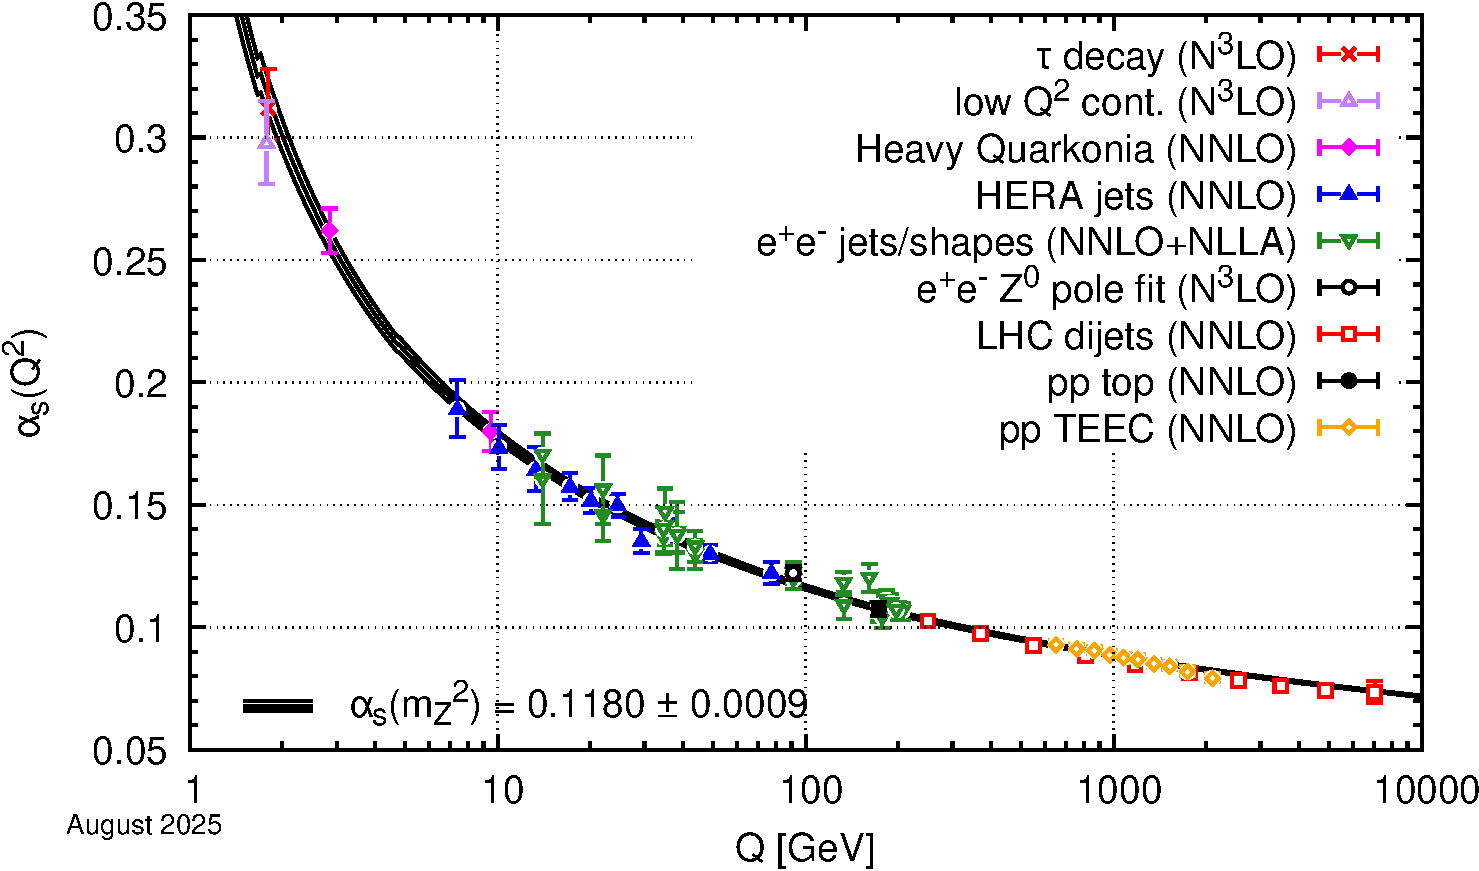
\includegraphics[width=0.7\linewidth]{figures/alphas-v-Q-2025-cropped.pdf}
	\caption{Summary of determinations of \(\alpha_s\) as a function of the energy scale Q compared to
		the running of the coupling computed at five loops taking as an input the current Particle Data Group (PDG) world average, \(\alpha_s(m_Z^2) = 0.1180 \pm 0.0009\) \cite{ParticleDataGroup:2026aaa}}
	\label{fig:runningCoupling}
\end{figure}

\begin{equation}
	\alpha_s(Q^2) = \frac{\alpha_s(Q_0^2)}{1 + \beta_0(\alpha_s(Q_0^2))\ln(Q^2/Q_0^2) + \mathcal{O}(\alpha_s^2)}
	\label{eq:alphasVsQ2}
\end{equation}

%At an energy scale \(Q\), consider a dimensionless observable \(X\). Lets assume that \(Q\) is sufficiently high that the quark masses become negligible in comparison. To calculate \(X\) as a perturbation series in the QCD coupling \(\alpha_s = \frac{g^2}{4\pi}\) (analogous to the QED fine structure constant), we need to remove ultraviolet divergences through renormalization. Renormalization introduces another arbitrary energy scale $\mu$ where the divergences are subtracted.  In general, \(X\) would depend on the ratio \(Q^2/\mu^2\) and post-renormalization coupling $\alpha_s(\mu^2)$. However, any physical observable should be independent of $\mu$:
%\begin{align}
%	\mu^2\frac{d X(Q^2/\mu^2, \alpha_s(\mu^2))}{d\mu^2} &= \left[\mu^2\frac{\partial}{\partial\mu^2} +  \mu^2\frac{\partial\alpha_s(\mu^2)}{\partial\mu^2}\frac{\partial}{\partial\alpha_s}\right] X(Q^2/\mu^2, \alpha_s(\mu^2)) = 0 \notag\\
%	\implies & \left[-\frac{\partial}{\partial t} + \beta(\alpha_s) \frac{\partial}{\partial\alpha_s}\right] X(e^t, \alpha_s) = 0.
%	\label{eqn:renormX}
%\end{align} 
%
%Where, \(t = \ln{\frac{Q^2}{\mu^2}}\), \(\beta(\alpha_s) = \mu^2\frac{\partial\alpha_s}{\partial\mu^2}\), \(\alpha_s\equiv\alpha_s(\mu^2(t))\)
%\begin{align}
%	\beta(\alpha_s) &= -\frac{\partial\alpha_s}{\partial t} \implies  t =  \int^{\alpha_s(Q^2)}_{\alpha_s}\frac{d\alpha_s}{\beta(\alpha_s)}\notag\\
%	\implies & \frac{\partial\alpha_s(Q^2)}{\partial t} = Q^2\frac{\partial \alpha_s}{\partial Q^2}  =  \beta(\alpha_s(Q^2)), \quad\frac{\partial\alpha_s(Q^2)}{\partial\alpha_s} = \frac{\beta(\alpha_s(Q^2))}{\beta(\alpha_s)}
%	\label{eq:runningCouplingIntro}
%\end{align}
%
%Substituting in Eq. \ref{eqn:renormX}, we see that \(X(1, \alpha_s(Q^2))\) is a valid solution. Thus the scale dependence in \(X\) comes from the \emph{running coupling} \(\alpha_s(Q^2)\).  Perturbatively expanding \(\beta(\alpha_s)\), we can write the \emph{renormalization group equation} as,
%
%\begin{align}
%	Q^2\frac{\partial \alpha_s}{\partial Q^2}  = -\alpha_s^2(Q^2)\left(\beta_0 + \beta_1\alpha_s(Q^2) + \mathcal{O}(\alpha_s^2(Q^2))\right)
%	\label{eq:RGEquation}
%\end{align}
%
%Where,
%\begin{equation}
%	\beta_0 = \frac{1}{(4\pi)^2}\left(11 - \frac{2}{3}N_f\right), \quad \beta_1 =  \frac{1}{(4\pi)^4}\left(102 - \frac{38}{3}N_f\right)
%\end{equation}
%
%
%
%Integrating Eq. \ref{eq:RGEquation}
%\begin{align}
%	\ln(\frac{Q^2}{Q_0^2})  &= \int^{\alpha_s(Q^2)}_{\alpha_s(Q^2_0)}\frac{d\alpha_s}{\beta(\alpha_s)}\notag\\
%	\implies \alpha_s(Q^2) &= \frac{\alpha_s(Q_0^2)}{1 + \beta_0(\alpha_s(Q_0^2))\ln(Q^2/Q_0^2) + \mathcal{O}(\alpha_s^2)}
%	\label{eq:runningCouplingRel}
%\end{align}
%
%Usually, the reference scale \(Q_0^2\) is set to a convenient energy scale in the perturbative regime. \(\alpha_s\) at all other scales can be inferred accordingly. Usually, \(Q_0\) is set to mass of the \(Z\)-boson, \(m_Z\) as shown in Fig. \ref{fig:runningCoupling}. Another approach is to choose a scale parameter, \(\Lambda\) such that \(\alpha_s(\Lambda) \rightarrow \infty\).  
%
%\begin{align}
%	\ln(\frac{Q^2}{\Lambda^2}) &= - \int_{\alpha_s(Q^2)}^{\infty} \frac{d\alpha_s}{\beta(\alpha_s)}  \notag\\
%	\implies \alpha_s(Q^2)  &= \frac{1}{\beta_0\ln(Q^2/\Lambda^2)}\left[1 - \frac{\beta_1}{\beta_0}\frac{\ln(\ln(Q^2/\Lambda^2))}{\ln(Q^2/\Lambda^2)} + \mathcal{O}\left(\frac{1}{\ln(Q^2/\Lambda^2)^2}\right)\right]
%	\label{eq:runningCouplingLambda}
%\end{align}
%\(\Lambda\) is called the \emph{confinement scale}, around \(200~\mathrm{MeV}\). 
%
Eq. \ref{eq:alphasVsQ2} show a monotonically decreasing relationship between \(\alpha_s\) and \(Q^2\). 
%
At high momentum transfers (\(Q \gg \Lambda\)), the coupling strength vanishes ($\alpha_s \to 0$). 
%
In this regime, quarks and gluons behave as quasi-free particles, making perturbative QCD (pQCD) calculations highly reliable (\emph{Asymptotic Freedom}).  
%
At low energy scales (\(Q \ll \Lambda\)), the coupling diverges. 
%
In this non-perturbative QCD (npQCD) limit, isolated color charges cannot exist and partons are permanently bound into color-neutral hadrons (\emph{Color Confinement}).

\subsection{Quark Gluon Plasma (QGP)}
\label{sec:QGPIntro}
Asymptotic freedom of QCD means that matter at extremely high temperatures and densities (high \(Q^2\)) undergo a \emph{deconfinement} phase transition, with partonic degrees of freedom replacing hadronic degrees of freedom. 
%
This state of deconfined quarks and gluons is called QCD/quark-gluon plasma due to analogous phenomena observed in atomic physics~\cite{SHURYAK198071}.

Thermodynamically, when temperature (\(T\)) or baryon number density (\(n_\mathrm{B}\)) approaches the confinement scale \(\Lambda\) introduced in Sec.~\ref{subsec:runningCoupling} (\(T \sim \Lambda \sim \mathcal{O}(10^{12})K,~\text{and}~n_\mathrm{B} \sim \Lambda^3 \sim 1~\text{fm}^{-3}\)) the boundaries between hadrons become ill defined resulting in hadrons ``melt'' into QGP~\cite{Fukushima_2010}.  
%
For reference, the core of our sun ``only'' has \(T\sim \mathcal{O}(10^{7})K\) and \(n_\mathrm{B}\sim\mathcal{O}(10^{-14})\text{fm}^{-3}\). 

These orders of \(T\) and \(n_\mathrm{B}\) are the theorized conditions prevalent in the universe a few \(\mu\mathrm{s}\) after Big-Bang. The only natural phenomena in the present-day, cold universe that can achieve these conditions are the cores of neutron stars~\cite{Annala_2020} or neutron star mergers~\cite{neutronStarMerger}. Artificially, the required  \(T\) and \(n_\mathrm{B}\) can be achieved at facilities like the Large Hadron Collider (LHC) and Relativistic Heavy Ion Collider (RHIC) through collisions of heavy-ions (like Au, Pb, etc.) at near-light speeds, the aptly named \emph{little bangs}. More on this will be discussed in Sec. \ref{sec:heavyIonCollisions}. 


\section{Hadronization and event generators}
\label{sec:eventGenerators}
Coherent branching does not only suppress soft emission, it also organizes the color flow of the shower.
%
Eq.~\ref{eq:coherentPattern} of shows that a pair of partons close in angle radiates as its parent, carrying the parent's charge, so the color of a branching is handed down the tree along with its momentum.
%
Applying this at every branching down to the cut-off \(t_0\), neighbouring partons are the ones that are color connected, and the final state has sorted itself into color singlet groups whose invariant masses are set by \(t_0\) and \(\Lambda\), and not by the scale of the hard process that started it.
%
This property is called \emph{preconfinement}~\cite{Ellis_Stirling_Webber_1996}.
%
The preconfined singlets can either decay directly into hadrons, giving the \emph{cluster} models~\cite{Webber:147786}, or stretch a confining color flux tube between color connected partons and break it up, giving the \emph{string} models~\cite{ANDERSSON198331}. 

QCD event generators chain these processes, matrix elements for the hard processes from eq.~\ref{eq:factorization}, parton showers, additional semi-hard scatterings among the remaining constituents of the incoming hadrons making up the \emph{underlying event}, hadronization, and finally the decays of unstable hadrons.
%
Everything below the hard process carries parameters that are not fixed by theory, and a set of values for them obtained by fitting to data is called a \emph{tune}.
%
Two generators starting from the same matrix element can therefore still disagree, and the spread between them is the usual way of gauging how much of a prediction is genuinely perturbative. 

This thesis uses PYTHIA~\cite{Sj_strand_2006} and HERWIG~\cite{Bellm:2015jjp}, which differ in how they deal with the coherence of Sec.~\ref{sec:coherentPartonBranching}.
%
HERWIG orders its shower in angle and imposes Eq.~\ref{eq:angularOrdering} directly, then hadronizes the preconfined singlets as clusters.
%
PYTHIA instead orders in transverse momentum and radiates off color dipoles rather than off individual partons, which suppresses soft wide-angle emission without ordering in angle at all, and hadronizes with strings.
%

Both generators are used with tunes made for RHIC energies~\cite{Skands_2010, PhysRevD.105.016011, adkins2019studying}, as the tunes in widest use are fitted mostly to LHC data and overshoot the underlying event at \sPP{200}{GeV}.
%
PYTHIA-6 and PYTHIA-8 share the string hadronization and the transverse-momentum ordered shower, and differ mainly in their treatment of multiple parton interactions, color reconnection and beam remnants, all of which control the multiplicity and the soft, wide-angle part of an event.
%

Ch.~\ref{ch:jhcorr} also uses JEWEL~\cite{Zapp:2013vla}, which adds scattering of the shower partons off a thermal medium to this picture.
%
The response of the detector to the generated particles is simulated separately using GEANT~\cite{Brun:1987ma}, and Ch.~\ref{ch:methods} describes how its effects are taken back out of a measurement.

\section{Relativistic collisions of  nuclei}
\label{ch:hic}
Outgoing partons from hard processes undergo many successive splitting and fragmentation processes, becoming a collimated ``spray'' of hadrons called \emph{jets} which are detected as dense clustering of energy in calorimeters. 
%
In principle, a \emph{jet finding algorithm} should be able to faithfully get the kinematics of the initiating parton given the theory discussed in sec.\ref{sec:partonShower}, which show partons cleanly branching into partons and eventually fragmenting into final-state hadrons that can be traced back to the shower partons. 
%
However reality is rarely this straightforward. 
%
First, the fragmentation functions that connect the partons and final state hadrons cannot be calculated in experiments. 
%
Second, it is not trivial to establish connection between final state particles and initial state partons even at the parton level, before we have the complications from hadronization and detector level reconstruction. 
%
For example, in a clean reaction like \(e^+e^-\to q\bar{q}\). If one of the quark emits a gluon, then depending on the emission angle of the gluon, we might cluster 2 or 3 jets in the final state. We will further define jet finding in sec.~\ref{sec:jetAlgo}

As discussed in sec.~\ref{sec:QGPIntro}, collisions of heavy-ions at near-light speeds can create the conditions for forming QGP.
%
Sec.~\ref{sec:RHIC} discussed RHIC and sec.~\ref{sec:STAR} describe the STAR detector system. 
%
Before moving on to analyses of heavy-ion collisions, we need to establish a few more concepts. 
%
Nuclei like $\rm ^{197}_{79}Au$, $\rm ^{96}_{40}Zr$, $\rm ^{96}_{44}Ru$,  etc. are complex arrangements of protons and neutrons that have a multitude of non-trivial initial configurations leading up to their collisions which have significant effects on the final state particle distributions. 
%
Therefore, any measurement done using heavy-ion events need to report these initial configurations of the colliding nuclei. We discuss these in sec.~\ref{sec:heavyIonCollisions}. 



\section{Finding Jets}
\label{sec:jetAlgo}
To address the prevalent ambiguity of jet definitions, the Snowmass Accord~\cite{Berger:1992etd} stated that, experimental and theoretical measurements had to use the same jet finding algorithm on final state hadrons in order to be comparable. 
%
Thus clustered jets are not-quite the proxies for partons in the same way as parton showers, but regions in the final state phase space that are most likely to have contributions from parton showers. 
%
Even after we define a jet, another ambiguity comes from the decision of what constituents in the event must be used as inputs into the jet finding algorithm. Especially, in heavy-ion collisions jet-medium interactions make that choice non-trivial. For example, is a soft particle inside the jet cone coming from soft gluon radiation from the jet or the medium? Keeping these considerations in mind, a ``good'' jet finding algorithm is:
\begin{itemize}
	\item \emph{Collinear safe}, meaning  it would find the same jet with the same \(p_\mathrm{T, jet}\) regardless of  fragmentation details
	\item \emph{Infrared safe}, meaning  it would find the same jets, even in the presence of a
	large number of soft partons
\end{itemize}

The most commonly used family of infrared and collinear safe jet algorithms, sequentially recombines constituents in an event according to the following prescription:

\begin{enumerate} 
	\item For every pair of particles \(\{i,j\}\) with momenta \((\mathbf{p}_i, \mathbf{p}_j) \equiv \{(p_{\mathrm{T},i}, \eta_i, \varphi_i), (p_{\mathrm{T},j}, \eta_j, \varphi_j)\}\)
	\begin{equation}
		d_{ij} = {\mathrm {min}}(p_{T,i}^{2p},p_{T,j}^{2p})\frac{\Delta R_{ij}^2}{R^2},~\text{and}~d_{i} = p_{T,i}^{2p}
	\end{equation}
	%
	where, \(\Delta R_{ij}^2 = (\eta_i-\eta_j)^2+(\phi_i-\phi_j)^2\) is the \etaphi distance between particle \(i\) and \(j\). 
	%
	\(R\) is the resolution parameter of the algorithm, which decides the angular extent of clustered jets.
	%
	\item $i_\mathrm{min} = \min(\{d_{ij}\}\cup \{d_{i}\})$ is found.  
	%
	$d_\mathrm{min} \in \{d_{ij}\}$, the particles are combined into one jet candidate, adding their energies and momenta according to some \emph{recombination scheme}, and the first step is repeated.  
	\item  $d_\mathrm{min} \in \{d_{i}\}$, this is recorded as a final state jet candidate.  It is removed from the list and the first step is repeated. 
\end{enumerate}
These steps are iterated until no particles remain. 
%
This algorithm becomes the \emph{\(k_\mathrm{T}\) algorithm}~\cite{kTAlgorithm} for \(p=1\), \emph{Cambridge-Aachen}~\cite{CambAlgorithm} for \(p=0\) and the most widely used \emph{anti-\(k_\mathrm{T}\) algorithm}~\cite{antiKtAlgorithm} for \(p=-1\). 
%
\begin{figure}
	\centering
	
\includegraphics[width=0.7\linewidth]{jet_areas.pdf}
	\caption{Jet areas of one \textsc{Pythia}~8 $pp$ event at $\sqrt{s}=200$~GeV
		(Detroit tune) with the $k_{\rm T}$ (top left), Cambridge/Aachen (top right) and
		anti-$k_{\rm T}$ (bottom) algorithms, $R = 1$. Coloured regions are the three
		hardest jets, the same colour marking the same jet in every panel; other jets are
		grey. Circles are particles, their area growing with $p_{\rm T}$.}
	\label{fig:jetalgorithms}
\end{figure}
The difference in these algorithms are shown in fig.~\ref{fig:jetalgorithms}.  
%
The \emph{FastJet} library~\cite{Cacciari:2011ma} efficiently implements these algorithms and a few more, and is the de-facto standard in the High Energy Physics (HEP) community. 
%
It also provides various recombination schemes. 
\begin{itemize}
	\item \emph{E-scheme}, just adds the four momenta of the jet candidates.  it is the default in FastJet and the most commonly used.
	\item \emph{Boost-invariant $p_t$/$p_t^2$/$E_t$/$E_t^2$ schemes} involve a preprocessing stage rescaling the energy to be equal to the 3-momentum for the
	$p_t$ and $p_t^2$ schemes or the 3-momentum to be equal to
	the energy in the $E_t$ and $E_t^2$ schemes. Then for all schemes the
	recombination $p_r$ of $p_i$ and $p_j$ is a massless 4-vector
	satisfying
	\begin{subequations}
		\begin{align}
			p_{t,r} &= p_{t,i} + p_{t,j}\,,\\
			\varphi_r &= \frac{w_i \varphi_i + w_j \varphi_j}{w_i + w_j}\,,\\
			y_r &= \frac{w_i y_i + w_j y_j}{w_i + w_j}\,,
		\end{align}
	\end{subequations}
	where $w_i$ is $p_{t,i}$ for the $p_t$ and $E_t$ schemes, and is
	$p_{t,i}^2$ for the $p_t^2$ and $E_t^2$ schemes. 
	\item \emph{Winner-takes-all (WTA) scheme} uses the four momentum of the higher momentum jet candidate
\end{itemize}

\section{Heavy-Ion Collisions}
\label{sec:heavyIonCollisions}

\begin{figure}
	\centering
	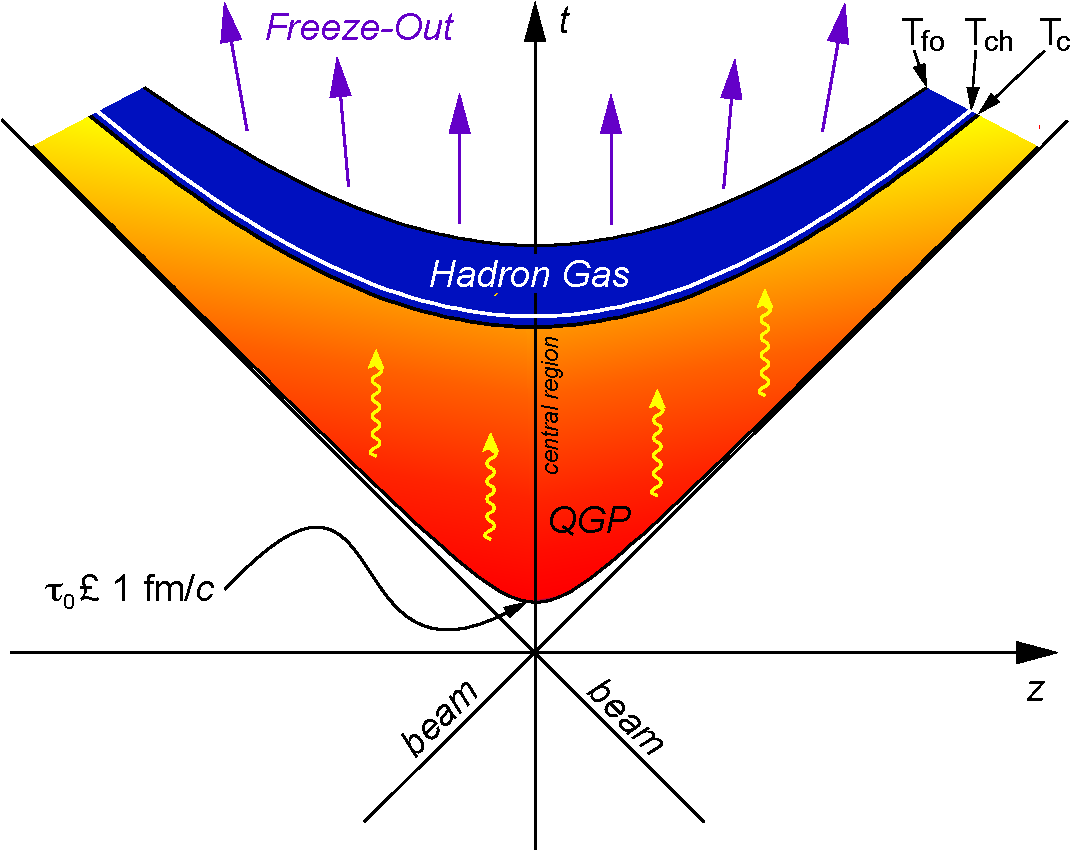
\includegraphics[width=0.7\linewidth]{figures/LightCone1_color-crop}
	\caption{A light cone diagram showing the stages of a heavy ion collision.  The abbreviation  $T_{\mathrm fo}$ is for the thermal freeze-out temperature, $T_{\mathrm ch}$ is for the chemical freeze-out temperature, and $T_{\mathrm c}$ is for the critical temperature where the phase transition between a hadron gas and a QGP occurs.  $\tau_0$ is the formation time of the QGP. Taken from~\cite{Connors_2018}}
	\label{fig:lightcone}
\end{figure}

Estimates of the energy density indicate that heavy ion collisions at RHIC and LHC  reach energy densities ranging between 1-12 GeV/fm$^3$~\cite{PhysRevC.93.024901,PhysRevC.94.034903}, well in excess of the 0.2-1 GeV/fm\(^3\) required for QGP formation~\cite{PhysRevD.90.094503, Karsch2002}. 
%

%\subsection{Space-time picture of QGP}
\label{sec:qgpSpacetime}
The heavy ion collision and the evolution of the fireball, as depicted in Figure~\ref{fig:lightcone}, has several stages, and the measurement of the final state particles can be affected by one or all of these stages depending on their production mechanism and interaction time within the medium. 
%
Immediately after the collision, the system is in a non-thermalized, pre-equilibrium state where, partons undergo hard scattering, dominated by \(2\to 2\) QCD processes with the outgoing partons back-to-back in azimuth (\(\Delta \varphi \approx \pi\)). 
%
At \(\tau \approx 0.5 - 1~\text{fm}/c\), the system thermalizes into the QGP state which expands following hydrodynamic laws. 
%
During the expansion, the system cools down until it reaches the temperature (\(T_c \approx 156\)~MeV from lattice QCD studies) at which a crossover phase transition to a hadronic gas state occurs. 
%
By \(\tau \approx 10~\text{fm}/c\) after the collision, confinement is restored and colored partons hadronize into colourless hadrons.
%
When the chemical freeze-out temperature (\(T_{ch} \approx 165\)~MeV) is reached, the particle abundances of the system are frozen. 
%
Elastic interactions can still occur till the kinetic freeze-out (\(T_{fo} \approx 100\)~MeV), where the particle momentum spectra are established.


%\begin{figure}[h]
%	\centering
%	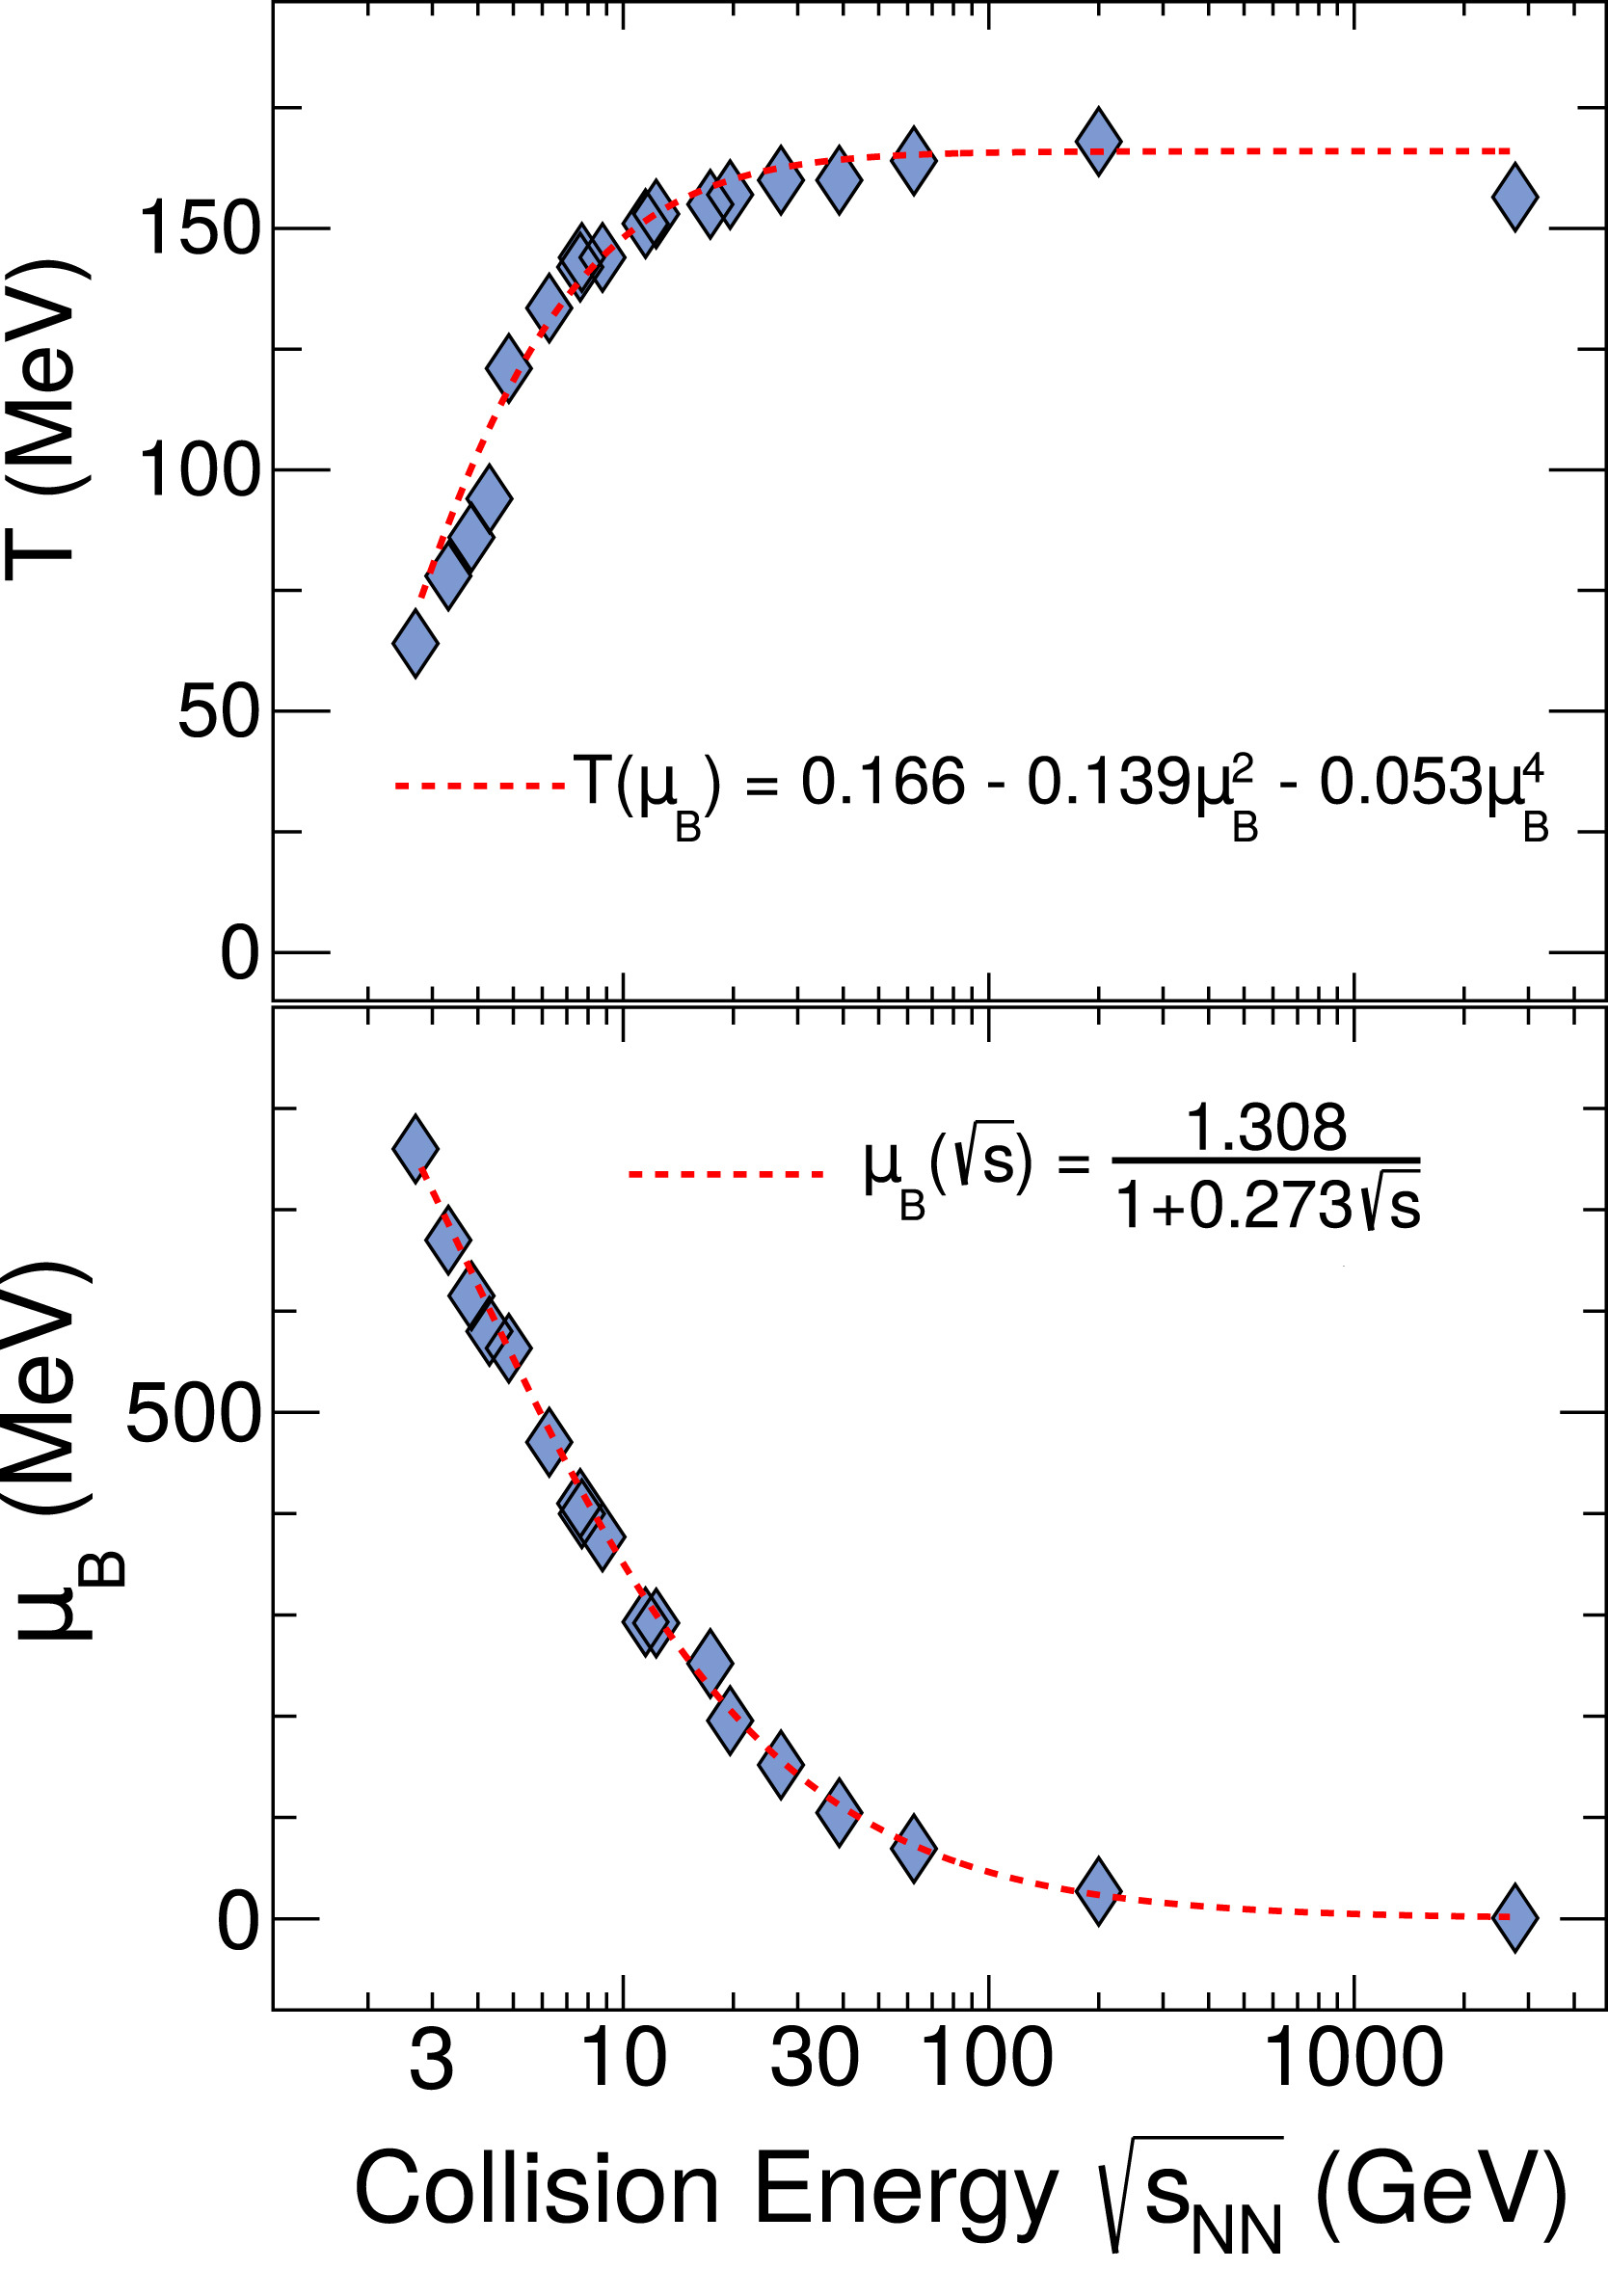
\includegraphics[width=0.5\linewidth]{figures/T_mu_vs_sNN}
%	\caption{Chemical freeze-out parameters \(T\) and \(\mu_\mathrm{B}\) obtained by thermal model fits to experimental data on particle yields as a function of collision energies. Red line represents parametrizations of \(T\) and \(\mu_\mathrm{B}\) as a function of $\sqrt{s_\mathrm{NN}}$}
%	\label{fig:tmuvssnn}
%\end{figure}
\subsection{Initial State of Colliding Nuclei}
The initial state of the incoming nuclei is not precisely known, but its properties impact the production of final state particles.  
%
The incoming nuclei are often modeled as either an independent collection of nucleons called a Glauber initial state~\cite{Miller:2007ri}, or a wall of coherent gluons called a Color Glass Condensate~\cite{IANCU2001583}. 
%
The widely used model for determining these quantities is the Glauber Monte Carlo (Glauber MC) model~\cite{Loizides_2015}, which assumes Wood–Saxon density distribution of nucleons.
%
The nuclei are then assigned a random impact parameter and translated to collide. 
%
If the distance between centers of nucleons is less than \(\sqrt{\sigma_\mathrm{inel}^\mathrm{NN}/\pi}\), where \(\sigma_\mathrm{inel}^\mathrm{NN}\) is the inelastic nucleon–nucleon cross section, the nucleons have undergone a binary collision. 
%
Nucleons that have undergone at least one binary collision are said to have participated in the reaction.
%
This procedure is followed to obtain the number of participant nucleons (\(N_\mathrm{part}\)) and the number of binary collisions (\(N_\mathrm{coll}\)) event-by-event.

A schematic diagram of the geometry of heavy-ion collisions is shown in Fig. \ref{fig:hictikz}. 
\begin{figure}
	\centering
	\begin{tikzpicture}
		\def\N{85} % number of nucleons
		\def\R{1.0} % nucleus radius
		\def\Nlay{5} % number of rings/layers
		\def\xs{0.25} % horizontally scale
		\def\Rp{0.92} % length photon
		\def\D{3.7} % horizontal distance between nuclei
		\pgfmathsetmacro\H{1.10*\R} % vertical distance between nuclei
		\pgfmathsetmacro\v{0.25*\D} % length vector
		
		%\message{^^J PbPb collision with impact parameter}
		
		% NUCLEUS
		% participants: nucleons in the vertical band where the two nuclei overlap
		\pic[xscale=\xs,nucleus participants,nucleus ymin=-\R,nucleus ymax=\R-\H] (L) at (-\D/2, \H/2) {nucleus};
		\pic[xscale=\xs,nucleus participants,nucleus ymin=\H-\R,nucleus ymax=\R] (R) at ( \D/2,-\H/2) {nucleus};
		
		% VELOCITY VECTORS
		\draw[vector] (L-0)++(2pt,0) --++ (\v,0); %node[above=2pt] {$v\approx c$};
		\draw[vector] (R-180)++(-2pt,0) --++ (-\v,0); %node[above=2pt] {$v\approx c$};
		
		% PHOTONS
		\foreach \ang in {60,90,120,-60,-90,-120}{
			\draw[photon] (L-\ang) --++ (\ang:\Rp);
			\draw[photon] (R-\ang) --++ (\ang:\Rp);
		}
		
		% MEASURES
		\draw[<->,thick]
		(R-0)++(0.3*\R,0) --++ (0,\R) node[midway,right] {$R\sim A^{1/3}\mathrm{fm}$};
		\draw[<->,thick]
		(0,-\H/2) -- (0,\H/2) node[midway,right] {$b$};
		%\node at (0.3*\D,0.7*\H) {$b > 2R$};
		
	\end{tikzpicture}
	\caption{Typical heavy-ion collision with an impact parameter of \(b\). The participating nuclei are colored red and the spectators are colored blue.}
	\label{fig:hictikz}
\end{figure}

\subsection{Centrality Determination} \label{sect:CentEP}
\begin{figure}[h]
	\label{fig:centralityVsNch}
	\centering
	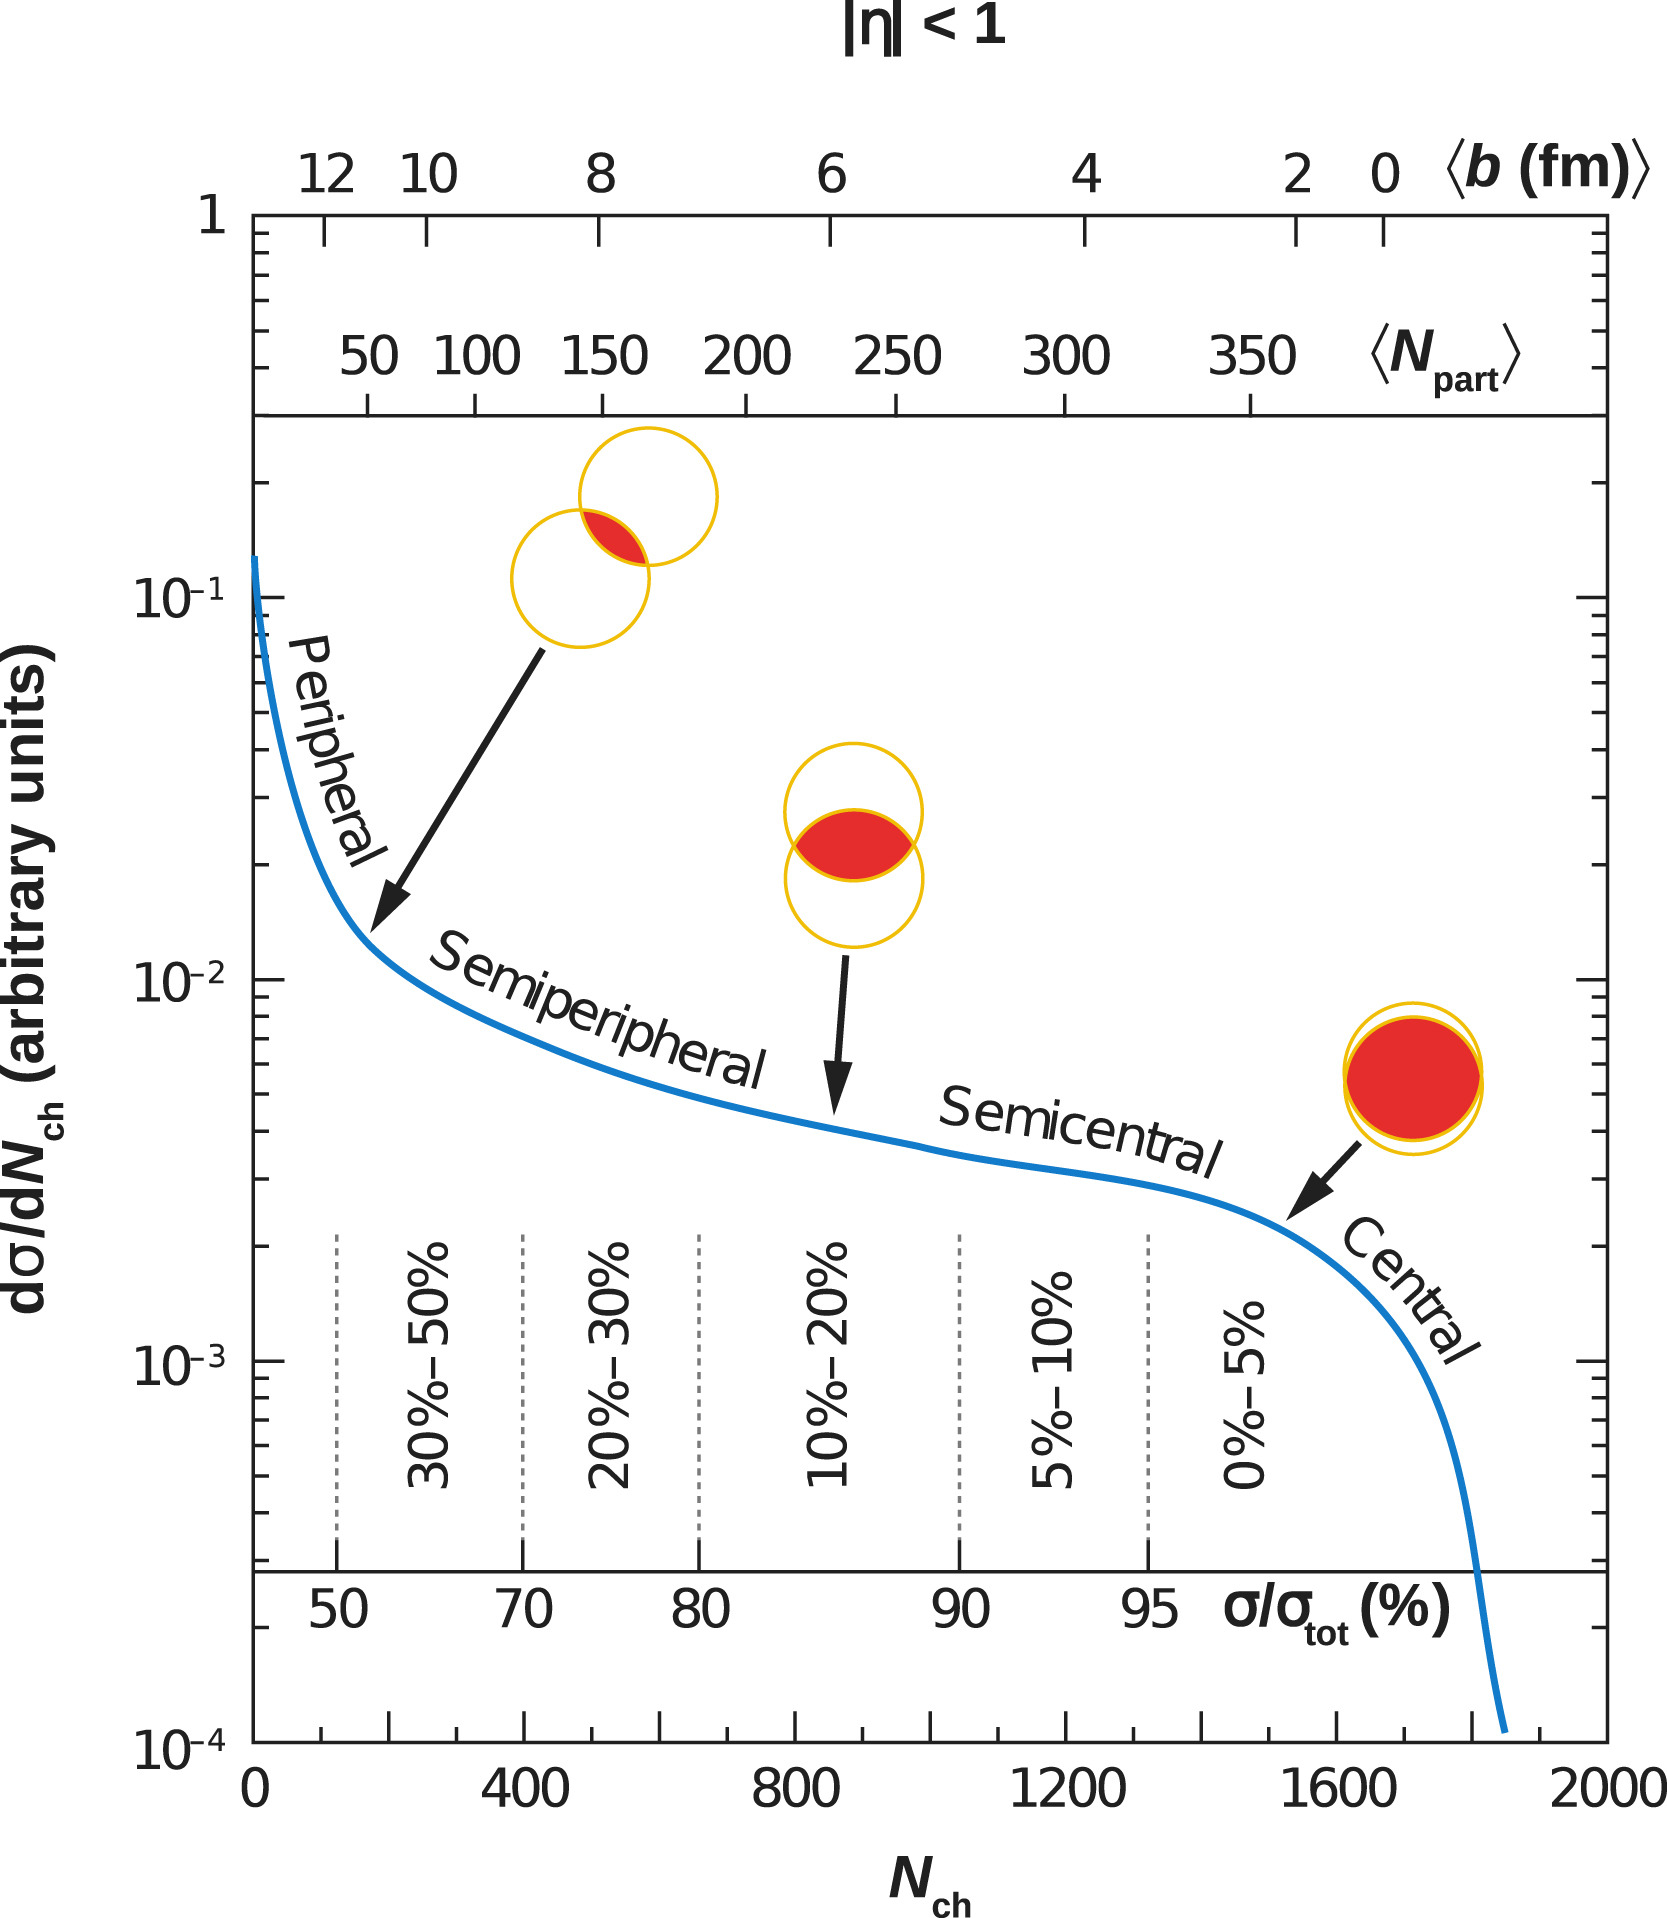
\includegraphics[width=0.6\textwidth]{figures/centrality_refmult.jpg}
	\caption{An illustration of the total inclusive charged particles multiplicity \(N_\mathrm{ch}\) and number of participant (\(N_\mathrm{part}\)) and impact parameter (\(b\)) in heavy-ion collisions. Taken from~\cite{Miller:2007ri}}
\end{figure}
As the impact parameter  (\(b\)) of collisions, the distance between the geometrical centers of the colliding nuclei, is not measurable in experiments, a proxy called \emph{centrality} is defined. 
%
Centrality is characterized by the charged particle multiplicity of events, connected to the impact parameter through a simulation defining it as a function of \(N_\mathrm{part}\), \(N_\mathrm{coll}\) 
and impact parameter \(b\) from Glauber model is mapped with the experimental data through a particle production model called the Two-Component Model~\cite{KHARZEEV2001121}. 
%
Assuming that particle production is governed by contribution from hard component (\(\propto N_\mathrm{coll}\)) and soft component (proportional to  \(\propto N_\mathrm{part}\)), it simulates the multiplicity distribution according to
\begin{equation}
	\frac{dN_\mathrm{ch}}{d\eta} = n_{pp}\left[xN_\mathrm{coll} + (1-x)\frac{N_\mathrm{part}}{2}\right]
\end{equation}
where the quantity \(n_{pp}\) is the multiplicity from a \(p+p\) collision of the same center-of-mass energy. \(x\) is the contribution of hard component. 
%
\(n_{pp}\) is drawn from a negative binomial distribution with parameters \(\text{NBD }(n_{pp}; \langle n_{pp}\rangle,k)\), where \( \langle n_{pp}\rangle\) is the average multiplicity in the \(p+p\) collision and \(k\) is the width of the distribution. 
%
The simulated charged multiplicity distribution is then fitted with the corresponding multiplicity distribution from the experiment. \(\langle n_{pp}\rangle\), \(k\), and \(x\) are kept as free parameters in the fitting to experimentally measured charged particle multiplicity distribution. 																		
%
Initial guess values for \(x\) could be set close to those determined in different experiments for faster convergence of fitting~\cite{back2004collision,PhysRevC.88.044909}. 

An event belongs to a centrality class, say 0\%–5\% if its charged particle multiplicity falls in the top \(5^\text{th}\) percentile. 
%
Fig.~\ref{fig:centralityVsNch} illustrates collision centrality definition in heavy-ion collisions by comparing the charge particle multiplicities with Glauber MC + Two-component model simulation.
%
Centrality classes are classified for the simulated distribution. 
%
\(\langle N_\mathrm{part}\rangle\), \(\langle N_\mathrm{coll}\rangle\) in those centrality classes are calculated. 

\subsection{Anisotropic flow}
\begin{figure}[h]
	\centering
	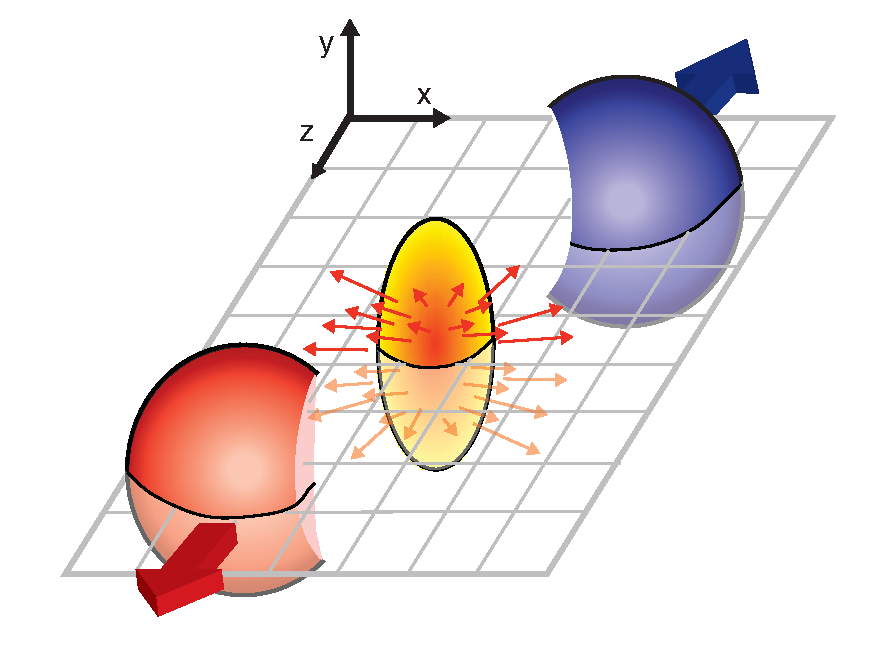
\includegraphics[width=0.4\textwidth]{figures/flow_elliptic_init_v4.pdf}
	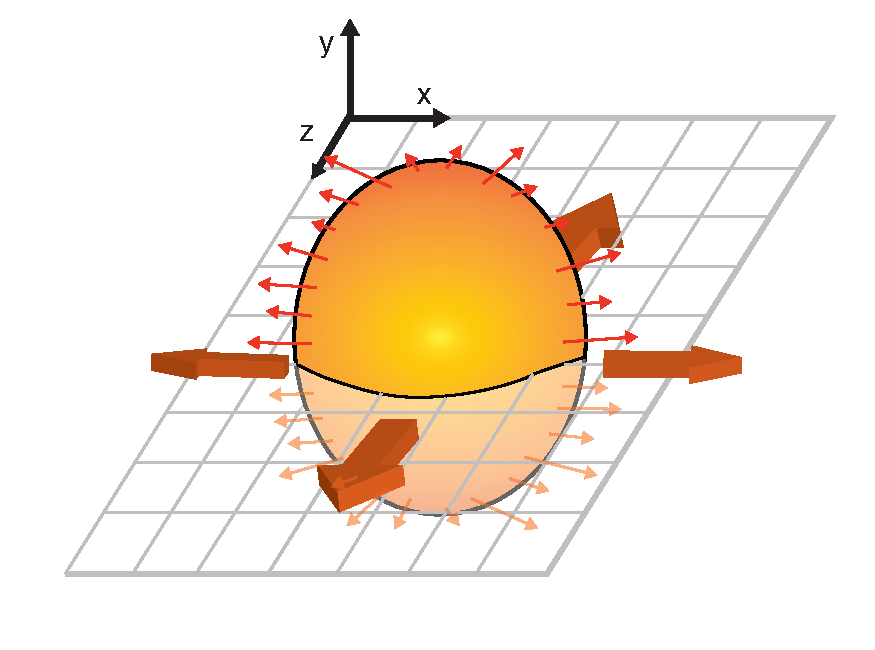
\includegraphics[width=0.4\textwidth]{figures/flow_elliptic_expd_xyz_v2.pdf}
	\label{fig:anisotropycartoon}
	\caption{Schematic diagrams showing the initial overlap region (left) and the spatial anisotropy generated by this anisotropic overlap region.  This anisotropy can be quantified using the Fourier coefficients of the momentum anisotropy. Taken from~\cite{Connors_2018}}
\end{figure}
Contrary to initial naive expectations of a gas-like QGP, the QGP formed in these collisions was shown to behave like a liquid of quarks and gluons~\cite{Heinz_2013}.
%
Thus, mean free path of particles in QGP fireball is much smaller than the fireball's system size.
%
Hence, in non-central heavy ion collisions the initial state coordinate space asymmetry generates a pressure gradient in the direction of the impact parameter $b$, schematically shown in fig.~\ref{fig:anisotropycartoon}. 
%
This spatial asymmetry translates into a azimuthal momentum anisotropy as the system expands, meaning that particles are more likely to be emitted along the plane where the pressure gradients are the highest. 
%
This plane is defined by the beam axis and the impact parameter of the collision, and called the \emph{reaction plane} (\(\Psi_{\rm RP}\)).
%
The anisotropy can be characterized by the Fourier decomposition of the azimuthal particle distribution with respect to \(\Psi_{\rm RP}\)~\cite{Bielcikova:2003ku,Voloshin:1994mz}:
\begin{equation}
	\frac{dN}{d(\phi - \Psi_{RP})} = \frac{N_0}{2\pi} \left( 1 + 2 \sum_{n=1}^{\infty} v_n \cos[n(\phi - \Psi_{RP})] \right),
	\label{fourier_azi_part_distr}
\end{equation}
%
The \emph{anisotropic flow} coefficients $v_{n}$, the $n^{\rm th}$ order term in the Fourier decomposition of the final state particle azimuthal distribution is given by,
%
\begin{equation}
	\label{flow}
	v_{n} = \left< \cos([n(\phi - \Psi_{\rm RP})]) \right>
\end{equation}
%
Due to the symmetry of the collision geometry, the most prominent contribution is from the second order coefficient $v_2$, called \emph{elliptic flow}.

\begin{figure}[h]
	\centering
	
\includegraphics[width=0.41\linewidth]{AnisotropyWithNoScaling (1).png}
	
\includegraphics[width=0.52\linewidth]{Gen1_IdentifiedParticle_v2.png}
	\caption{\textbf{Left panel}: Elliptic flow $v_2$ for several particle species in Au + Au collisions at \sNN{200}{GeV}  from STAR and PHENIX experiments. Predictions from hydrodynamic models are shown as lines. Taken from \cite{GYULASSY200530}. \textbf{Right panel}: Number of constituent quarks ($n_q$) scaled $v_2$ as a function of $p_{\rm T}/n_q$. Taken from \cite{Sorensen_2006}.}
	\label{fig:AnisotropyResults}
\end{figure}

$v_2$ was measured by the STAR and PHENIX for several particle species and is shown in Fig. \ref{fig:AnisotropyResults}. 
%
Large positive $v_2$ values indicate collective phenomena associated with a strongly coupled fluid, or a \emph{signature of QGP}.
%
A scaling of the $v_2$ values with the number of constituent quarks (2 for mesons, 3 for baryons) yielded a universal curve as a function of $p_{\rm T}/n_q$ suggesting the flow dynamics were developed in a medium with quark and gluon degrees of freedom, i.e. QGP.

\subsubsection{Event plane reconstruction}
\label{sec:EP_Recon}
The reaction plane, \(\Psi_{\rm RP}\) cannot be directly measured and is approximated by the second-order symmetry plane, $\Psi_{2,EP}$, referred to as the \emph{event plane}  in this text, for simplicity.  
%
\(\Psi_{\rm RP} \to \Psi_{2, EP}\) if nucleon distributions were in their average positions and devoid of fluctuations from interactions among nucleons~\cite{PhysRevC.101.064901}.
%
By measuring the charged particle azimuthal distribution, the n-th order event plane can be extracted by~\cite{Poskanzer:1998yz},  
%
\begin{equation}
	\Psi_{n,EP} = \frac{1}{n} \arctan \left(\frac{Q_{y, n}}{Q_{x, n}} \right),
	\label{eqn:EP}
\end{equation}
%
the weighted vector \(\mathbf{Q}_n = Q_{x, n}\hat{\mathbf{x}}+ Q_{y, n}\hat{\mathbf{y}}\) are given by,
%
\begin{align}
	\mathbf{Q}_n = \hat{\mathbf{x}}\sum_{\mathrm{tracks}} p_{\rm T, track} \cos (n \phi_{\rm track}) + \hat{\mathbf{y}}\sum_{\mathrm{tracks}} p_{\rm T, track} \sin (n \phi_{\rm track}).
	\label{Eqn:Qvecs}
\end{align}
%
where the sum is calculated for all reconstructed charged particles (tracks) in the event, $\phi_{\rm track}$ is the track's azimuthal angle, and $p_{\rm T, track}$ the track's transverse momentum.  
%

Due to finite acceptance and multiplicities, the calculated event plane has an underlying anisotropy that is corrected by applying two separate correction methods.  
%
First, a calibration and recentering correction procedures are applied to remove bias introduced by non-uniform acceptance of the TPC tracking system and further account for potential beam-condition effects~\cite{Barrette:1997pt,PhysRevC.55.1420,Poskanzer:1998yz}.  
%
This procedure involves recentering the weighted $\mathbf{Q}_2$-vectors such that, $\langle\mathbf{Q}_2 \rangle = \mathbf{0}$. 
%
It is done by calculating a modified $\mathbf{Q}_2$, obtained by subtracting an event averaged $\langle\mathbf{Q}_2 \rangle$ from each event's nominal $\mathbf{Q}_2$.
%

The higher harmonics of $\Psi_{n,EP}$ still persist after recentering \cite{Poskanzer:1998yz}, and are removed through a second correction step, referred to as  the shifting method, applied event-by-event  to make the event-plane angle isotropic in the lab frame \cite{Voloshin:2008dg}. 
%
This method defines a new angle:
%
\begin{equation}
	\Psi'_{2,EP} = \Psi_{2,EP} + \sum_n \frac{2}{n}
	(- \langle \sin (n\Psi_{2,EP}) \rangle \cos(n\Psi_{2,EP}) + \langle \cos(n\Psi_{2,EP}) \sin(n\Psi_{2,EP}) \rangle) ,
	\label{eqn:Shift}
\end{equation}
%
Usually 20 orders of Fourier moment are removed. 
%
Additional details of the recentering and shifting corrections can be found in Refs.~\cite{Wang:2012bga,Barrette:1997pt,Poskanzer:1998yz}

The difference between $\Psi_{RP}$ and \(\Psi_{2, EP}\) is quantified by event-plane resolution, $R_n$ or $R_n\{\Psi_{2, EP}\}$ given by Eqn.~\ref{resolution}. 
%
The observed $v_n$, $v_n^{\rm obs}$ is corrected for this limited resolution by doing, $v_n = v_{n}^{\rm obs}/R_n$ \cite{Abbas:2013taa,Poskanzer:1998yz}.  
%
\begin{equation}
	R_n = R_n\{\Psi_{2, EP}\} = \langle \cos(n[\Psi_{RP} - \Psi_{2, EP}]) \rangle \qquad \text{$n$ is even}
	\label{resolution}
\end{equation}

Furthermore, individual events are divided into two random sub-events by assigning charged tracks to sub-events, ``$a$" and ``$b$". 
%
The sub-events are unique, with approximately equal multiplicities. 
%
We can write the correlation of two event planes by taking the product of two sub-events, \cite{Barrette:1996rs,Poskanzer:1998yz}
%
\begin{equation}
	\langle \cos(n[\Psi_{2, EP}^{a} - \Psi_{2, EP}^{b}]) \rangle = 
	\langle \cos(n[\Psi_{2, EP}^{a} - \Psi_{RP}]) \rangle
	\langle \cos(n[\Psi_{2, EP}^{b} - \Psi_{RP}]) \rangle,
	\label{resolution2sub}
\end{equation}
%
This allows calculation of the event-plane resolution directly from data. Since $a$ and $b$ have equal multiplicities, the resolution of each sub-event can be calculated from the correlation between the two sub-events as \cite{Poskanzer:1998yz}:

\begin{equation}
	\langle \cos(n[\Psi_{2, EP}^{a} - \Psi_{RP}]) \rangle = 
	\sqrt{\langle \cos(n[\Psi_{2, EP}^{a} - \Psi_{2, EP}^{b}]) \rangle} .
	\label{resolutionIndiv}
\end{equation}

The event-plane resolution is multiplicity dependent and calculated for separate ranges of collision centrality using the two sub-events method.  
%
Narrower bins are calculated and then combined accordingly to match the ranges required, by averaging the results from the narrow bins weighted by the multiplicity of each bin \cite{Voloshin:2008dg}.

\section{Jets in QGP}
As discussed in sec.~\ref{sec:qgpSpacetime}, hard scatterings of partons that produce jets happens before the system thermalizes into QGP (parton producing a 10~GeV jet scatters at \(\tau \sim 1/E \sim 0.2\text{fm}/c\)). 
%
Thus the ensuing parton shower traverses the QGP, and resulting jet is \emph{modified/quenched} compared to an appropriate \emph{baseline}. 
%
The two main mechanisms for jet quenching are \emph{collisional} and \emph{radiative} energy losses. 
%
Collisional energy loss happens due to the elastic scattering between the parton and the medium constituents and usually dominates for lower energy partons. 
%
Radiative energy loss happens due to induced gluon radiation (\textit{bremsstrahlung}) through inelastic scatterings with the medium particles \cite{MAJUMDER201141,QinWang2024,Burkeetal}. 
%
For partons with \ptGeq{parton}{5} , this is usually the dominant source of energy loss \cite{LandoltBornstein2010:sm_lbs_978-3-642-01539-7_16}. 
%
%\subsection{Combinatorial background in heavy-ion jets}
%Final state of heavy-ion collisions is characterized by a massive \emph{Underlying Event}, arising from the thermalized QGP. 
%%
%Although useful for bulk calculations like elliptic flow, including them in the jet clustering would artificially inflate the amount of radiation in the jet cone, as we generally want to restrict the jet constituents to remnants of a parton shower. 
%%
%This background is generally uncorrelated to the jet and hence called \emph{Uncorrelated/Combinatorial Background}.  
%%
%Heavy-ion jet background subtraction is quite an active field of study. 
%%
%The method of background subtraction is different for different jet analysis. 
%
%For 

%\subsection{Heavy-ion jet measurements}
The baseline measurement is done in a collision system where either QGP is not formed or has negligible lifetime compared to central heavy-ion collisions. 
%
Two possible choices arise for the baseline, first is \(p+p\) collisions from which we can calculate the \emph{Nuclear Modification Factor} (\RAA) for distributions of any observable \(\mathbf{O}\) calculated in \(p+p\) and \(A+A\) collisions,
given by
\begin{equation}
	R_{\rm AA}(\mathbf{O}, b) = \frac{dN_{\rm AA}/d\mathbf{O}}{\left<T_{\rm AA}(b)\right> . d^2\sigma_{pp}/d\mathbf{O}}
\end{equation}\label{RAA}
where $T_{\rm AA}(b) = N_{\rm coll}(b)/\sigma_{\rm NN}^{\rm inel}$ is the nuclear overlap function  which determines the number of participating nucleons and number of binary collisions $N_{\rm bin}$ for a heavy ion collision as a function of its impact parameter (\textit{b})~\cite{doi:10.1142/S0217751X95001467}.
%
The second common baseline used in absence of a \(p+p\) baseline is peripheral collisions of heavy-ion collisions. The \emph{Relative Nuclear Modification Factor} \(R_{CP}\) is given by,
%
\begin{equation}
	R_{CP}(\mathbf{O}, b) = \frac{dN/d\mathbf{O}}{\left< N_{\rm bin}(b) \right>} \biggm\lvert_{\rm cent} \times \frac{\left< N_{\rm bin}(b) \right>}{dN/d\mathbf{O}} \biggm\lvert_{\rm peri}
\end{equation}

\begin{figure}
	\centering
	
\includegraphics[width=0.8\linewidth]{Gen0_AngularCorrelation_JetQuenching.png}
	\caption{Measurement of the angular correlation between all charged hadrons and the leading hadron in the event for p + p (black lines), d + Au (red and green markers), and Au + Au events (blue markers), performed by the STAR experiment. The vanishing of the away-side yield around $\Delta\phi\approx \pi$ in Au + Au events is evidence of particles getting quenched in the QGP medium. Taken from \cite{Adams:2003im}.}
	\label{fig:angularcorr}
\end{figure}

Before infrastructure became available to reliably reconstruct a sufficient number of jets in heavy-ion collisions,  the effects of the medium on high energy partons were studying the \emph{Di-hadron correlation}. 
%
Leading hadron (highest $p_\mathrm{T}$ in event) is used as a jet proxy and the azimuthal angular correlation ($\Delta\varphi$) of all charged hadrons in the event is studied.
%
Fig. \ref{fig:angularcorr} shows one of the first measurements performed by STAR~\cite{Adams:2003im}, di-hadron correlations compared between p + p, Au + Au, and d + Au collisions. 
%
The p + p and d + Au both show peaks around $\Delta\varphi = 0$ and $\Delta\varphi =  \pi$ as expected, given that hard scatterings are dominated by \(2\to 2\) Feynman diagrams. 
%
However, for Au + Au collisions, the peak around $\Delta\varphi = \pi$ completely vanishes. 
%
This was the expectation because depending on the distance from the center of the collision where the initial back-to-back partons were produced, one of the partons would travel a larger distance in the QGP medium and therefore lose more energy than the other one.

\begin{figure}
	\centering
	
\includegraphics[width=0.8\linewidth]{Gen0_SingleParticle_RAA.png}
	\caption{Nuclear modification factor $R_{\rm AA}$ as a function of $p_\mathrm{T}$ for identified particle species in Au + Au collisions at \sNN{200}{GeV} measured by the PHENIX experiment. Taken from \cite{Tannenbaum_2015}.}
	\label{fig:singleparticleraa}
\end{figure}

A closer look at jet quenching was given by the PHENIX experiment through a collection of  \RAA~measurements discussed in eq.~\ref{RAA} for identified particles spectra, shown in Fig. \ref{fig:singleparticleraa}.
%
Whereas, direct photons ($\gamma$) do not interact strongly, and hence have no yield modification in the medium.
% 
All strongly interacting particles show varying levels of suppression from 0.2 - 0.6, again confirming their energy loss in the presence of QGP.

Although measurements with high $p_\mathrm{T}$ hadrons help us understand jet quenching mechanisms in the medium, they suffer from survival bias, as these hadrons arise from a subsample of jets which usually undergo the least amount of quenching \cite{PhysRevC.99.051901}. 
%
Fully reconstructed jets, however, are mostly unbiased probes of energy flow at high $p_\mathrm{T}$, and offer a wealth of substructure observables which allow us to look at energy flow within the jet more differentially.
%
This motivates the studies presented in chapters~\ref{ch:jhcorr} and~\ref{ch:angularities}.   

\begin{figure}
	\centering
	
\includegraphics[width=1\linewidth]{Gen1_ChargedParticleAndJets_RCP.png}
	\caption{$R_{CP}$ distributions for charged hadrons (open markers) and jets (solid markers) from RHIC (blue star markers) and LHC (red circle markers) experiments. Taken from \cite{STARChargedJet} and references within \cite{PhysRevLett.91.172302, ALICEChargedJet, ATLASChargedHadron}.}
	\label{fig:chargedparticlercp}
\end{figure}
The STAR experiment measured the \(R_{CP}\) of the $p_\mathrm{T}$ spectra of charged particle jets (clustered charged tracks only and contain no calorimeter hits (towers) as input) from central and peripheral Au + Au collisions at \sNN{200}{GeV} shown in fig.~\ref{fig:chargedparticlercp} \cite{STARChargedJet}. 
%
Measured for charged jets was compared to $R_{CP}$ for charged hadrons from STAR at the same energy, and to the measured $R_{CP}$ for charged hadrons and jets from the ALICE and ATLAS experiments at \sNN{2.76}{TeV}. 
%
First, the charged hadrons $R_{CP}$ is found to be the same over the same range of $p_\mathrm{T}$ at RHIC and LHC energies (which are an order of magnitude apart). 
%
The charged jet $R_{CP}$ is also found to have similar values between RHIC and LHC energies with roughly 60\% of the energy lost outside the jet cone in central collisions with respect to peripheral collisions, with no significant $p_\mathrm{T}$ dependence in contrast to the $p_\mathrm{T}$ dependence observed for the charged hadrons $R_{CP}$. 
%
This may be because the inclusive hadron distribution usually arises from the leading hadron in the corresponding jet, and is therefore is sensitive to the fragmentation function. 
%
This fragmentation process can therefore introduce the $p_\mathrm{T}$ dependence of $R_{CP}$ in hadrons. 

\begin{figure}
	\centering
	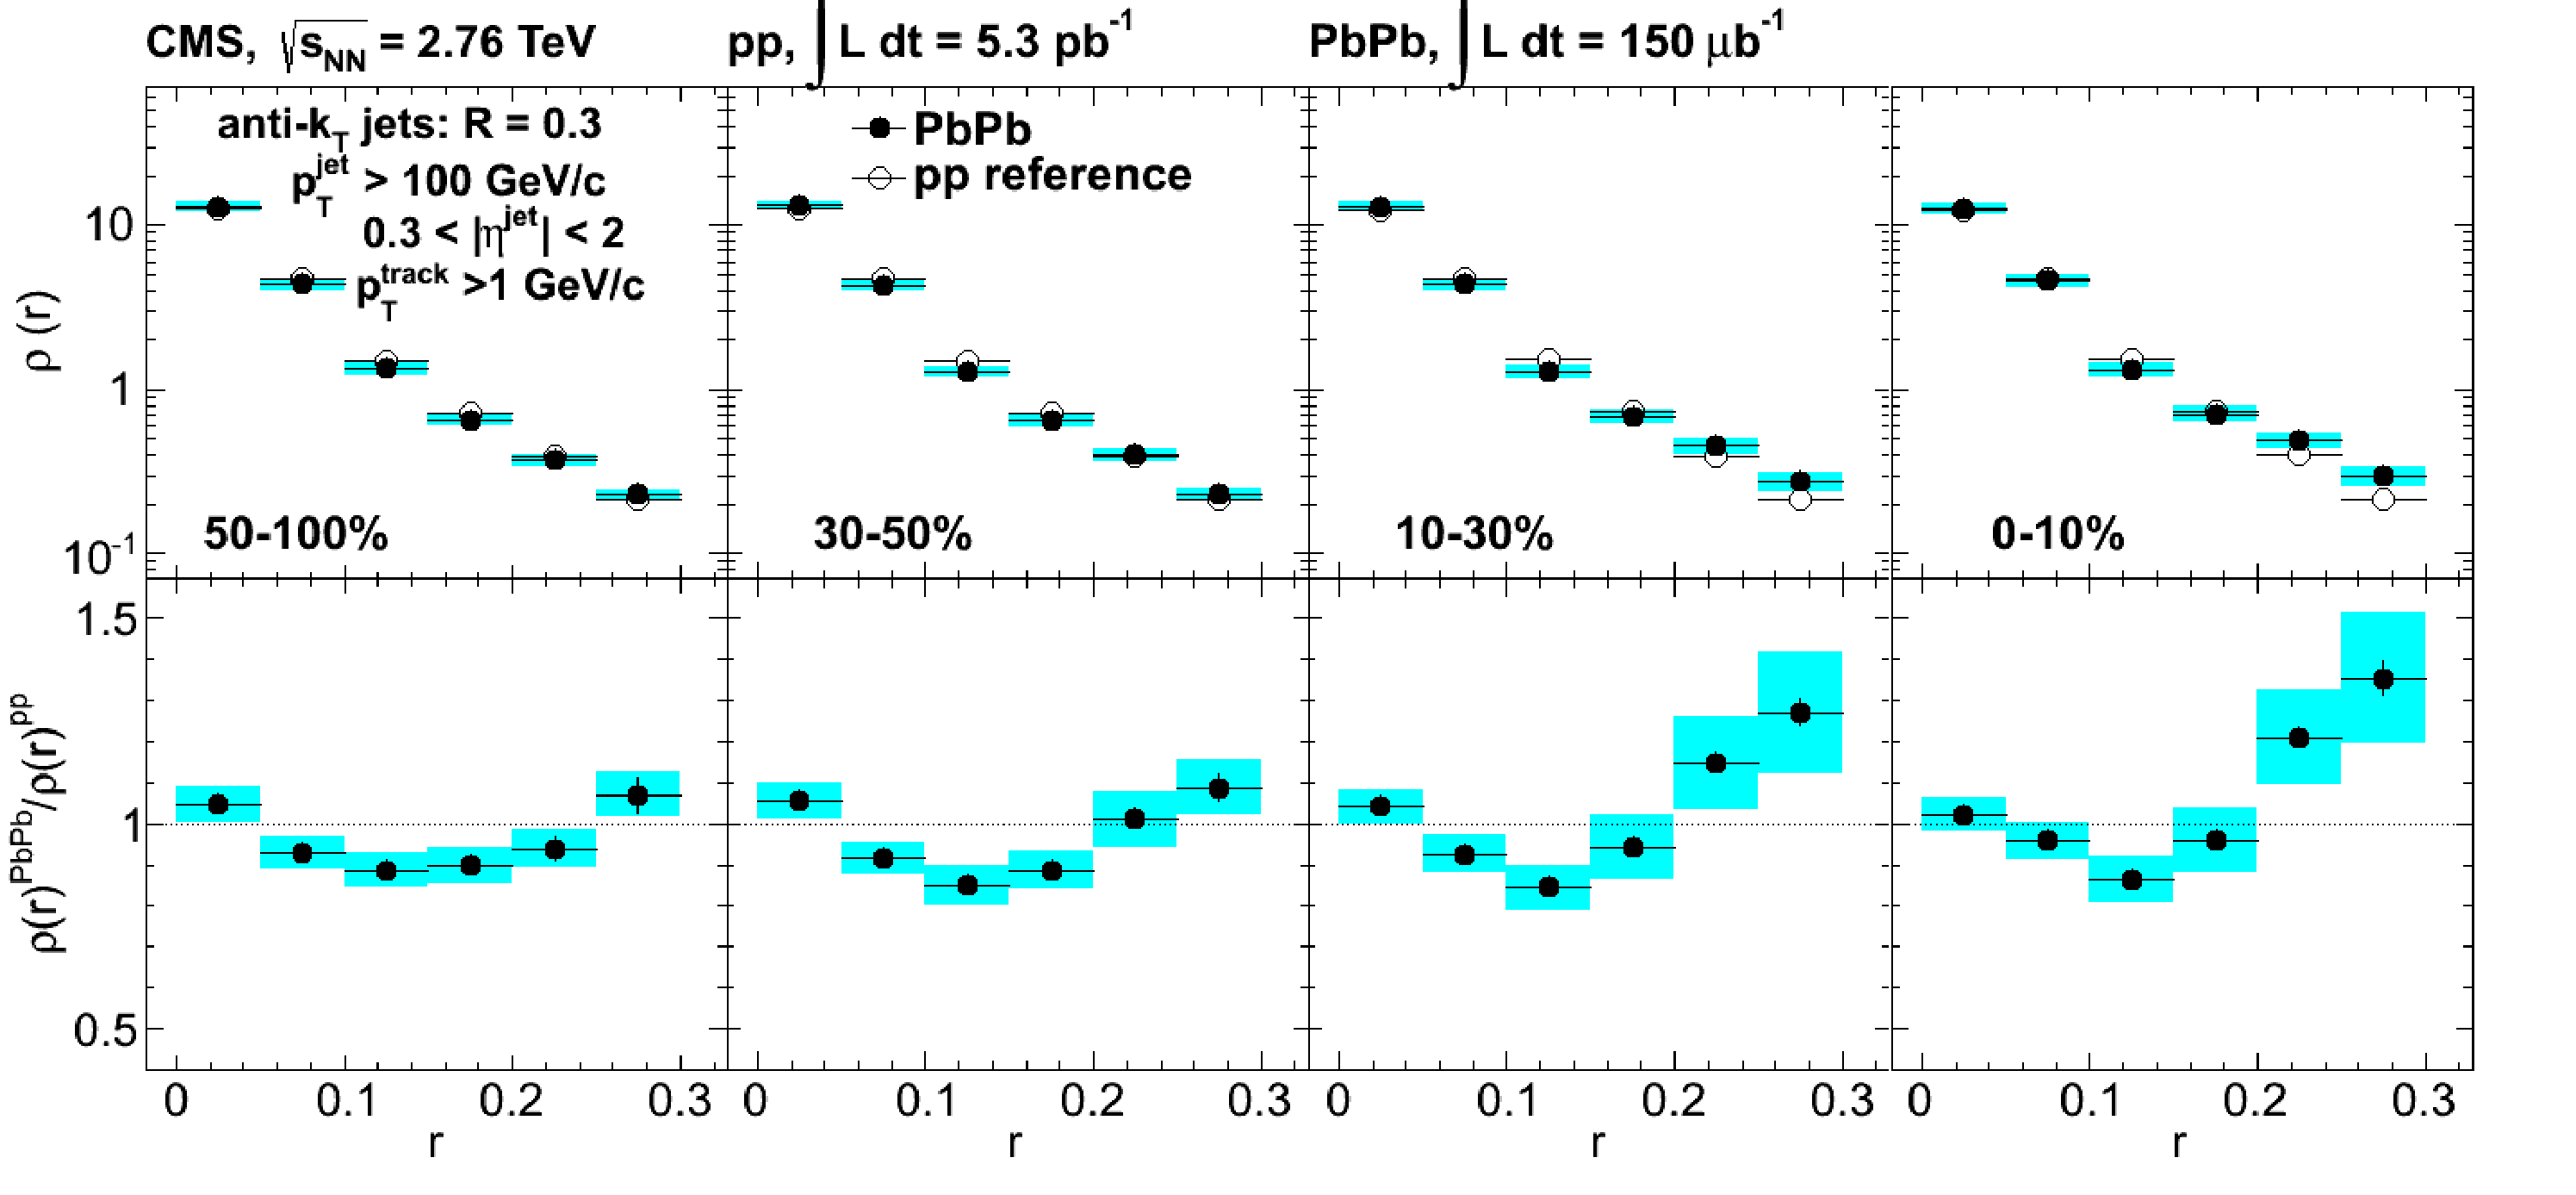
\includegraphics[width=\linewidth]{figures/CMSJetShapeFinalJS4Cent}
	\caption{Differential jet shapes in Pb+Pb and \(p+p\) collisions for four Pb+Pb  centralities. Each spectrum is normalized so that its integral is unity.  This shows that there are more particles in jets in central collisions and these modifications are primarily at large angles relative to the jet axis, as expected from partonic energy loss. Taken from~\cite{Connors_2018}}
	\label{fig:cmsjetshapefinaljs4cent}
\end{figure}
Going a bit into the jet substructure, CMS measurement of jet's average radial momentum profile around the jet-axis, called \emph{differential jet shape} defined as,
\begin{equation}
	\rho(r) = \frac{1}{\delta r} \frac{1}{N_{\mathrm jet}} \sum_{\mathrm jets} \frac{ \sum_{{\mathrm tracks} \epsilon [r_a, r_b)} p_{T}^{\mathrm track}}{p_{T}^{\mathrm jet}}
\end{equation}
%
where the jet cone is divided rings of width $\delta r$ which have an inner radius $r_a$ and an outer radius $r_b$.  
%
From the results shown in fig.~\ref{fig:cmsjetshapefinaljs4cent}, the differential jet shapes in the most central Pb+Pb collisions are broadened in comparison to measurements done in \pp collisions at the same center of mass energy ~\cite{Chatrchyan:1605718}.  
%
These measurements demonstrate that there is an enhancement in the modification with increasing angle from the jet axis, indicating a broadening of the jet profile and a depletion near r~$\approx$~0.2.

\section{Outline}
Angular ordering makes the angular distribution of energy inside a jet a record of the shower that produced it, with the wide-angle radiation coming from the early, hard splittings and the core of the jet being filled in later.
%
This thesis measures that distribution.
%
It is measured first in \pp collisions, where it is a test of the vacuum shower and a baseline, and then in \AuAu collisions, where a deviation from that baseline is the imprint of the medium the shower has gone through. 

Ch.~\ref{ch:STAR} describes RHIC and the STAR detector, in particular the TPC and the BEMC which measure the charged and neutral parts of a jet.
%
Ch.~\ref{ch:hic} defines jets as the output of a jet finding algorithm rather than as partons, introduces SoftDrop grooming, and sets up the quantities used to describe a heavy-ion collision: the Glauber picture of the initial state, centrality, the event plane, and the nuclear modification factors used to quantify jet quenching.
%
Ch.~\ref{ch:methods} collects the analysis techniques, mainly the classifiers used to tag jets and the unfolding procedure used to remove detector effects from a measured distribution.
%
Ch.~\ref{ch:jhcorr} presents jet-hadron correlations relative to the event plane in \AuAu collisions, which probe the dependence of energy loss on the path length traversed in the medium.
%
Ch.~\ref{ch:angularities} presents generalized angularities, inclusive and groomed, in \pp collisions and then in \AuAu collisions.
%
Ch.~\ref{ch:summary} summarizes both measurements and what they suggest about where to go next. 







%===========================================================================================


